The earlier Sections of this Chapter have covered the concepts and code related to program creation, but have not looked at how these concepts actually affect the computer when the program is run. This Section illustrates the actions that occur inside the computer when your program is executed. A good understanding of these concepts work will enable you to use them effectively.

This Section will help you answer the following questions:
\begin{itemize}
  \item What happens when the program is started?
  \item What happens when the code executes a procedure call?
\end{itemize}

\subsection{Starting a Program} % (fold)
\label{sub:starting_a_program}

Double clicking a program's icon, or launching it from the command line, causes the program to run. This is as much as most normal users need to know about using programs. However, as a Software Developer you need to know more about what is actually happening as you will be the one who defines what the computer does when your program runs.

\bigskip

Starting a program is the responsibility of the \emph{Operating System}. When the program is launched the following steps are performed. A discussion of each of these steps follows.

\begin{enumerate}
  \item Space is allocated in memory for the Program, and partitioned into areas for the program's \textbf{code}, and the call \textbf{Stack}.
  \item The program's code is loaded into memory, into the \textbf{code} Section.
  \item A \textbf{frame} is added to the \textbf{Stack} with the location of the first instruction in the program.
  \item The computer starts running the instructions based on the current frame in the stack.
\end{enumerate}

\clearpage
\subsubsection{Allocating Memory for the Program} % (fold)
\label{ssub:allocating_memory_for_the_program}

To start the program the Computer first needs to get the program's instructions into memory. This task is performed by the Operating System when the program is launched. The Operating System allocates memory for the program to use, and partitions this memory into different areas. Each area will be used to store different kinds of information needed by the program. An illustration of this is shown in Figure \ref{fig:program-creation-visualise-helloworld-1}.

\begin{figure}[htbp]
   \centering
   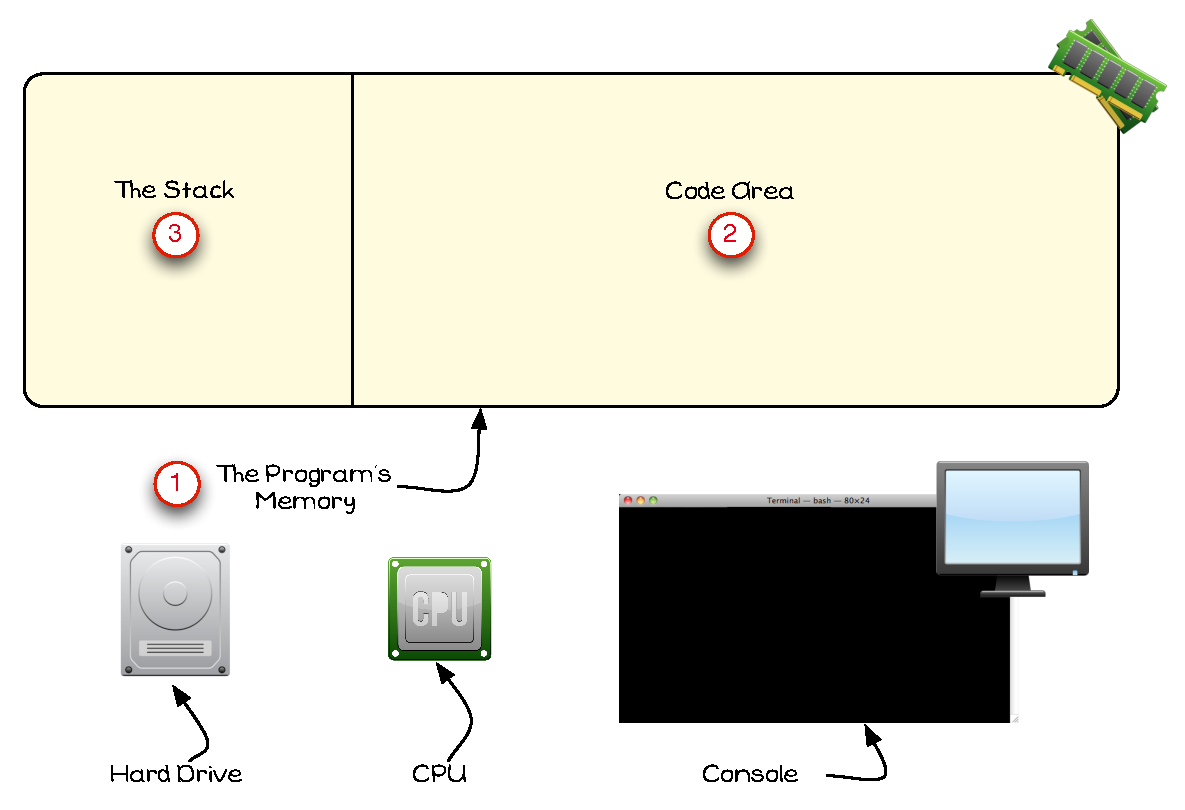
\includegraphics[width=\textwidth]{./topics/program-creation/images/ProgramExecution01} 
   \caption[Program Memory Space]{Operating System prepares memory for the Program}
   \label{fig:program-creation-visualise-helloworld-1}
\end{figure}

\mynote{
\begin{itemize}
  \item In Figure \ref{fig:program-creation-visualise-helloworld-1} the indicated areas show the following:
  \begin{enumerate}
    \item The Operating System allocates memory for the program.
    \item Part of the allocated memory will be designated to store the program's instructions. This can be thought of as the \emph{Code Area}.
    \item Another part of the allocated memory will be set aside to keep track of the current instruction. This area is called the \emph{Stack}.
  \end{enumerate}
\end{itemize}
}

% subsubsection allocating_memory_for_the_program (end)
\clearpage
\subsubsection{Loading the Code} % (fold)
\label{ssub:loading_the_code}

Having allocated the program some memory, and partitioned this space into the \textbf{Stack} and \textbf{Code} area, the Operating System then reads the program's instructions from the executable file and loads these into the Code area. This is illustrated in Figure \ref{fig:program-creation-visualise-helloworld-2}.

\begin{figure}[htbp]
   \centering
   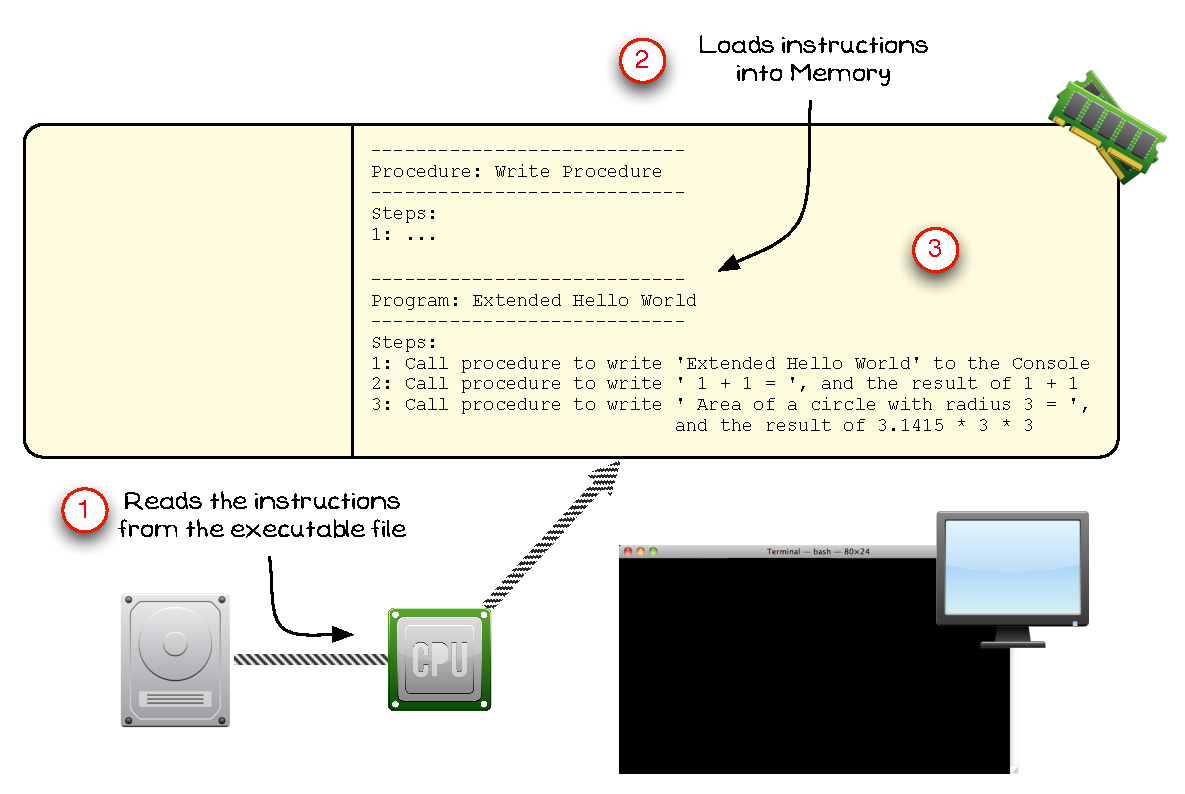
\includegraphics[width=\textwidth]{./topics/program-creation/images/ProgramExecution02} 
   \caption[Code loaded into memory]{The Operating System loads the program's code into memory}
   \label{fig:program-creation-visualise-helloworld-2}
\end{figure}

\mynote {
\begin{itemize}
  \item In Figure \ref{fig:program-creation-visualise-helloworld-2} the indicated areas show the following:
  \begin{enumerate}
    \item The program's instructions are read from the executable file the user launched.
    \item The instructions are stored into the program's memory: into the code area.
    \item When this finishes, all of the program's instructions are loaded into memory. In Figure \ref{fig:program-creation-visualise-helloworld-2} the instructions are shown as the pseudocode from Listing \ref{lst:program-creation-hello-pseudo}. In reality these will be the \emph{machine code} instructions that were saved into the executable file by the compiler.
  \end{enumerate}
  \bigskip
  \item The \emph{Operating System} is a software component that is used to control access to the hardware. In this case the Operating System takes the responsibility for setting up the machine so that it can run the program the user launched.
\end{itemize}
}
% subsubsection loading_the_code (end)

\clearpage
\subsubsection{Setting Up The First Instruction} % (fold)
\label{ssub:setting_up_the_first_instruction}

Now that the code is loaded into memory, the Operating System uses the details saved in the executable file to setup the program's first instruction. This will be loaded onto the Stack, which is responsible for keeping track of the current instruction. The compiler will have used the program's \textbf{entry point} to store these details when the program was compiled. This is shown in Figure \ref{fig:program-creation-visualise-helloworld-3}.

\begin{figure}[htbp]
   \centering
   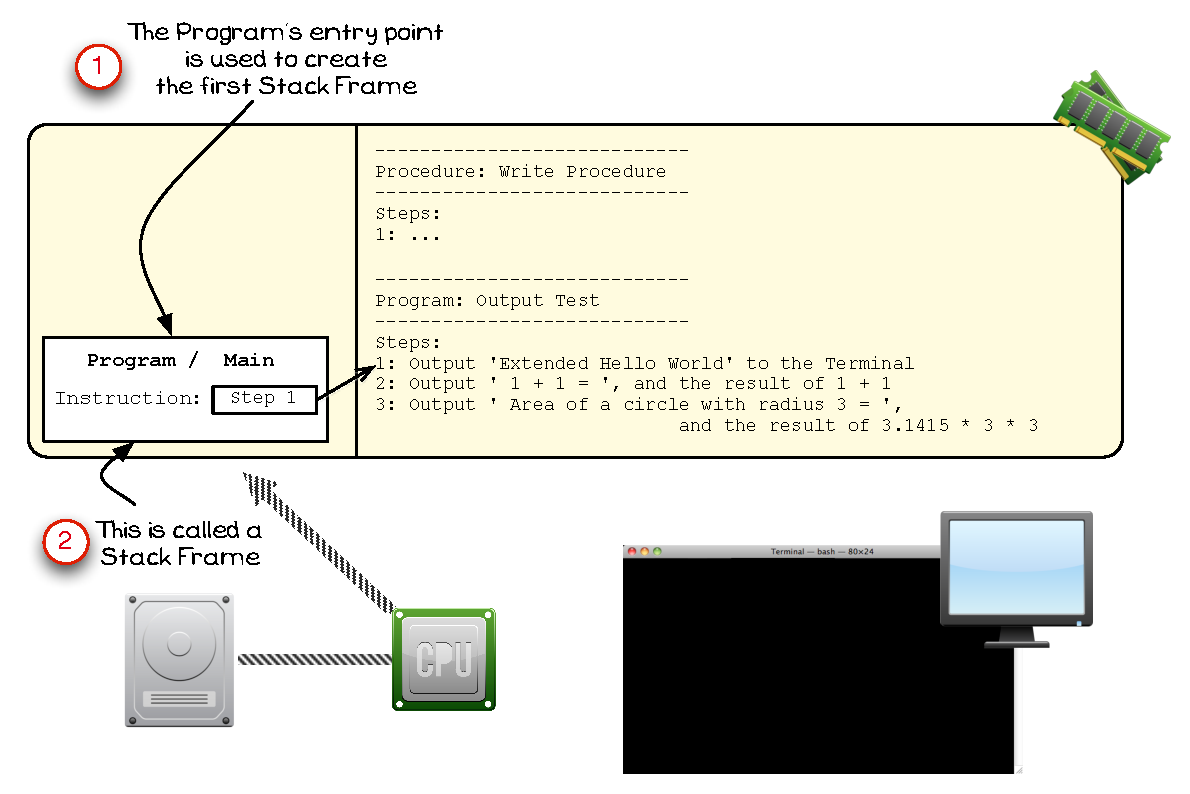
\includegraphics[width=\textwidth]{./topics/program-creation/images/ProgramExecution03} 
   \caption{The current instruction is loaded onto the Stack}
   \label{fig:program-creation-visualise-helloworld-3}
\end{figure}

\mynote {
\begin{itemize}
  \item In Figure \ref{fig:program-creation-visualise-helloworld-3} the indicated areas show the following:
  \begin{enumerate}
    \item The program's instruction is tracked on \emph{The Stack}.
    \item Each Stack Frame keeps a record of the current instruction within a Procedure. This area is called the Stack as the Frames are \emph{stacked} one on top of the other. The one on the top of the \emph{stack} tells the computer which instruction is to be run.
  \end{enumerate}
  \bigskip
  
  \item The Stack keeps track of the current instruction.
  \item The current instruction refers to the code loaded into the Code area.
  \item The compiler will have saved the details for which instruction is first into the executable file.
  \item In your code the program's \textbf{entry point} tells you which instruction will be first.
\end{itemize}
}

% subsubsection setting_up_the_first_instruction (end)

\clearpage
\subsubsection{Running The First Instruction} % (fold)
\label{ssub:running_the_first_instruction}

The Operating System has finally finished loaded the Program, and can now start its instructions running. The CPU uses the \textbf{Current Instruction} that is on the top of the Stack, locates the Code, and runs the instruction. In this case this is a procedure call to a Procedure that writes output to the Terminal. When this instruction completes, the text \emph{Output Test Program} will have appeared on the Terminal for the user to see. The results of this are shown in Figure \ref{fig:program-creation-visualise-helloworld-4}. 

\begin{figure}[htbp]
   \centering
   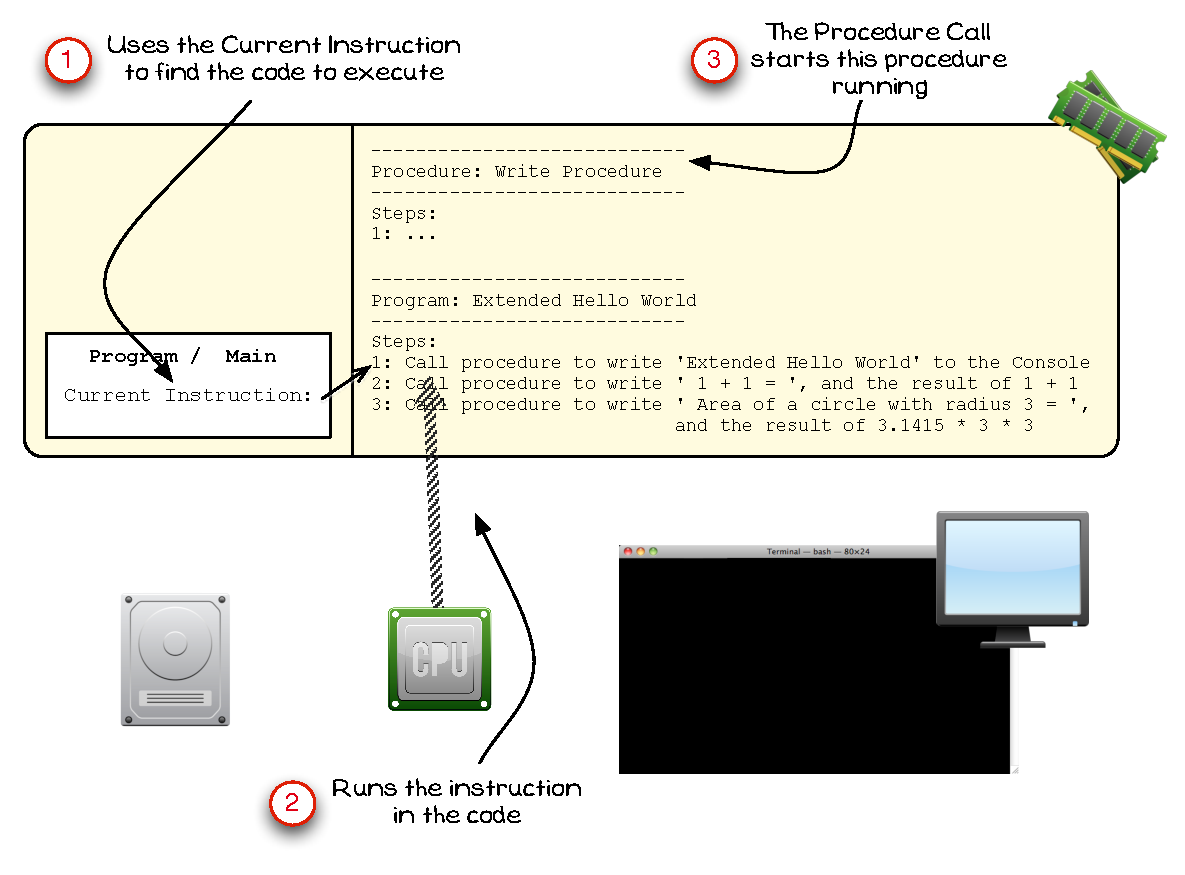
\includegraphics[width=\textwidth]{./topics/program-creation/images/ProgramExecution04} 
   \caption{The Computer runs the first instruction, outputting details to the Terminal}
   \label{fig:program-creation-visualise-helloworld-4}
\end{figure}


\mynote{
\begin{itemize}
  \item In Figure \ref{fig:program-creation-visualise-helloworld-4} the indicated areas show the following:
  \begin{enumerate}
    \item The current instruction is read from the Frame on the top of the Stack.
    \item The Computer runs the instruction from the code loaded into memory.
    \item The instruction is a procedure call, which starts the execution of the Write Procedure.
  \end{enumerate}
  
  \bigskip
  \item The computer runs the code \textbf{one} instruction at a time.
  \item When that instruction is finished it moves onto the next instruction. This is important, and means that are programs run the commands in \textbf{Sequence}.
  \item Writing data to the Terminal takes more than a single instruction, the procedure call gets the Computer to run the instructions in the called Procedure.
\end{itemize}
}

% subsubsection running_the_first_instruction (end)
% subsection starting_a_program (end)

\clearpage
\subsection{Calling the Write Procedure} % (fold)
\label{sub:calling_a_procedure}

At this point the Computer has been instructed to \texttt{Call the Write Procedure}. This procedure\footnote{The \texttt{printf} procedure in C and the \texttt{WriteLn} procedure in Pascal.} will output the data passed to it to the Terminal. In order to do this, the instructions within the called procedure need to be followed.

\subsubsection{Calling Write for the first time} % (fold)
\label{ssub:calling_write_for_the_first_time}

Each Procedure contains instructions that when followed get the Computer to perform a task. The procedure call sets up the Stack so that the instructions within the Write Procedure are executed.

\begin{figure}[htbp]
   \centering
   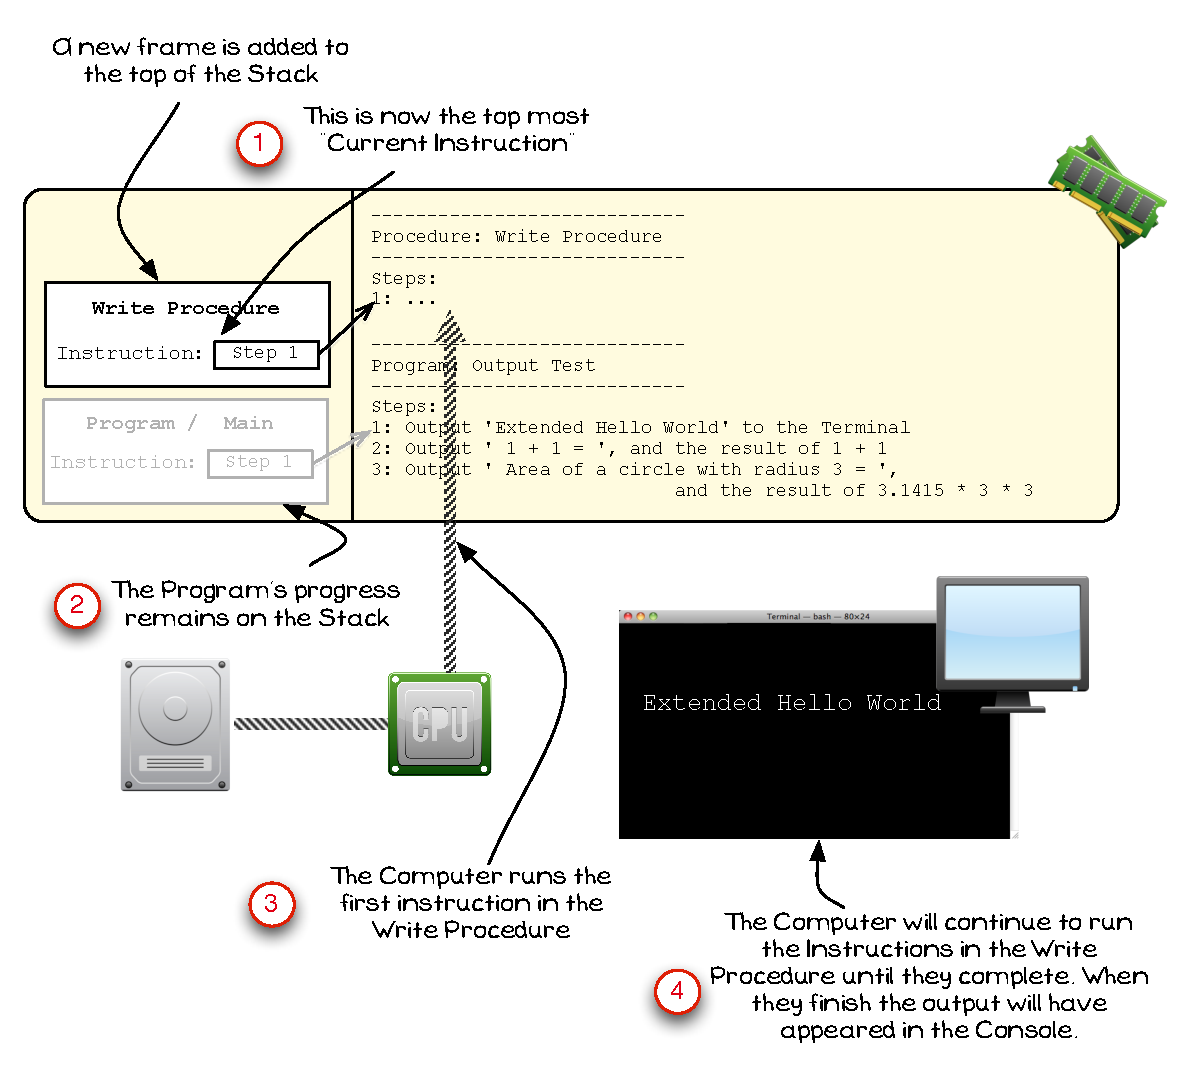
\includegraphics[width=0.9\textwidth]{./topics/program-creation/images/ProgramExecution05} 
   \caption{The Write Procedure is called, and has its instructions executed}
   \label{fig:program-creation-visualise-helloworld-5}
\end{figure}

\mynote{
\begin{itemize}
  \item In Figure \ref{fig:program-creation-visualise-helloworld-5} the indicated areas show the following:
  \begin{enumerate}
    \item A new Frame is added to the Stack for the Write Procedure.
    \item The new Frame appears on top of the Frame that has the program's Current Instruction.
    \item Now the Computer can run the instructions within the Write Procedure.
    \item The instructions are run one at a time until the Write Procedure finishes. At this time the first output will have appeared on the Terminal.
  \end{enumerate}
\end{itemize}
}


% subsubsection calling_write_for_the_first_time (end)
\clearpage
\subsubsection{The Write Procedure Ends} % (fold)
\label{ssub:the_write_procedure_ends}

When the Write Procedure's instructions finish control needs to return to the code that called it, in this case the program's code.

\begin{figure}[htbp]
   \centering
   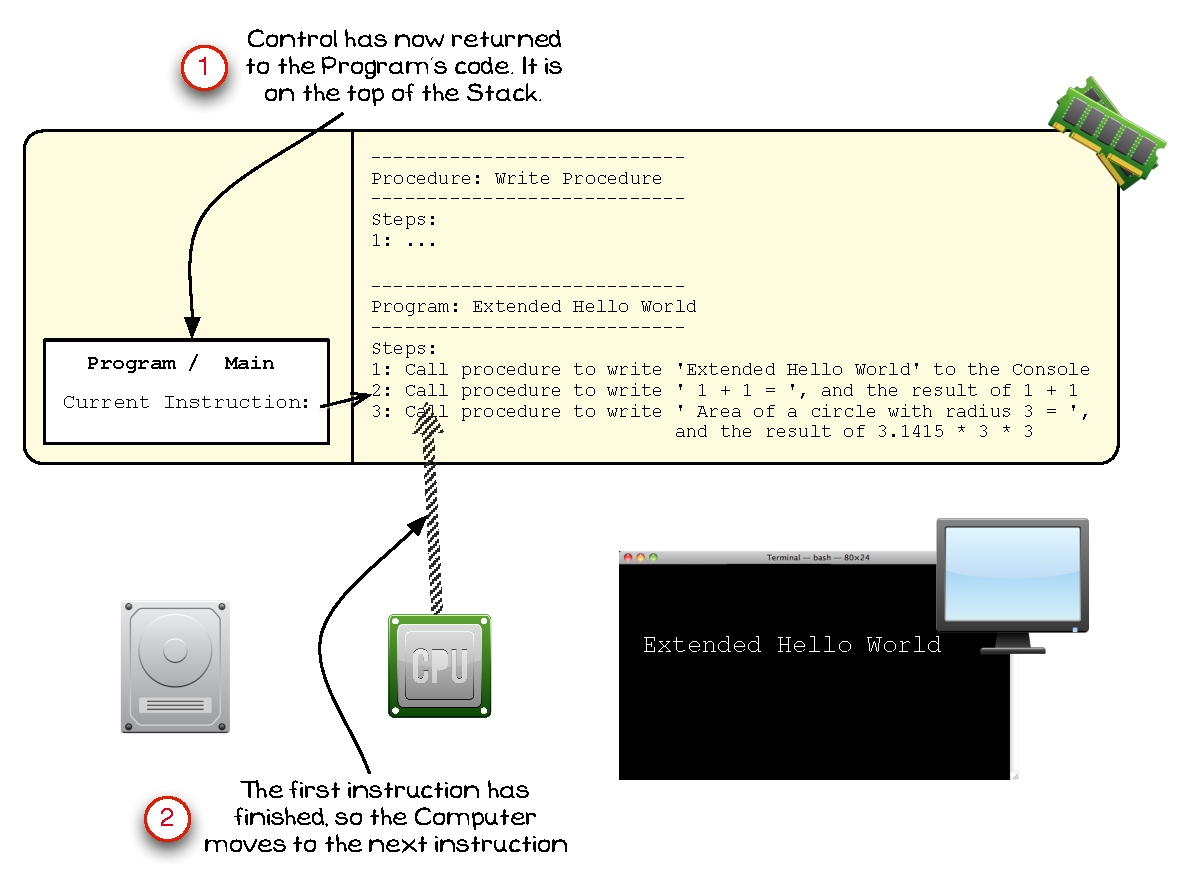
\includegraphics[width=\textwidth]{./topics/program-creation/images/ProgramExecution06} 
   \caption{The Write Procedure is called, and has its instructions executed}
   \label{fig:program-creation-visualise-helloworld-6}
\end{figure}

\mynote{
\begin{itemize}
  \item In Figure \ref{fig:program-creation-visualise-helloworld-6} the indicated areas show the following:
  \begin{enumerate}
    \item When the Write Procedure finishes its Frame is removed from the Stack, and control returns to the program's code.
    \item The first instruction on the program's code has now finished, so the Computer moves to the second instruction.
  \end{enumerate}
\end{itemize}
}

One way to visualise this is to picture the Program, and the Procedure, as a book of instructions. Imagine you are told to follow the instructions in a book. You get the book, place it on a table and read the first instruction which tells you to perform the \emph{Write Procedure}. You leave the original book on the table, and fetch the \emph{Write Procedure} book and place it on top of the book on the table, thereby creating a Stack of books. Now you can follow the instructions, one by one, from the book on top of the Stack. When you finish the last instruction you take the book off the top of the stack and return to the book beneath it. This will enable you to perform the steps within the Procedures without forgetting where you are up to in the earlier code.


% subsubsection the_write_procedure_ends (end)
\clearpage
\subsubsection{The Second Call to Write} % (fold)
\label{ssub:the_second_call_to_write}

The second instruction in the program's code is another call to the Write procedure.

\begin{figure}[htbp]
   \centering
   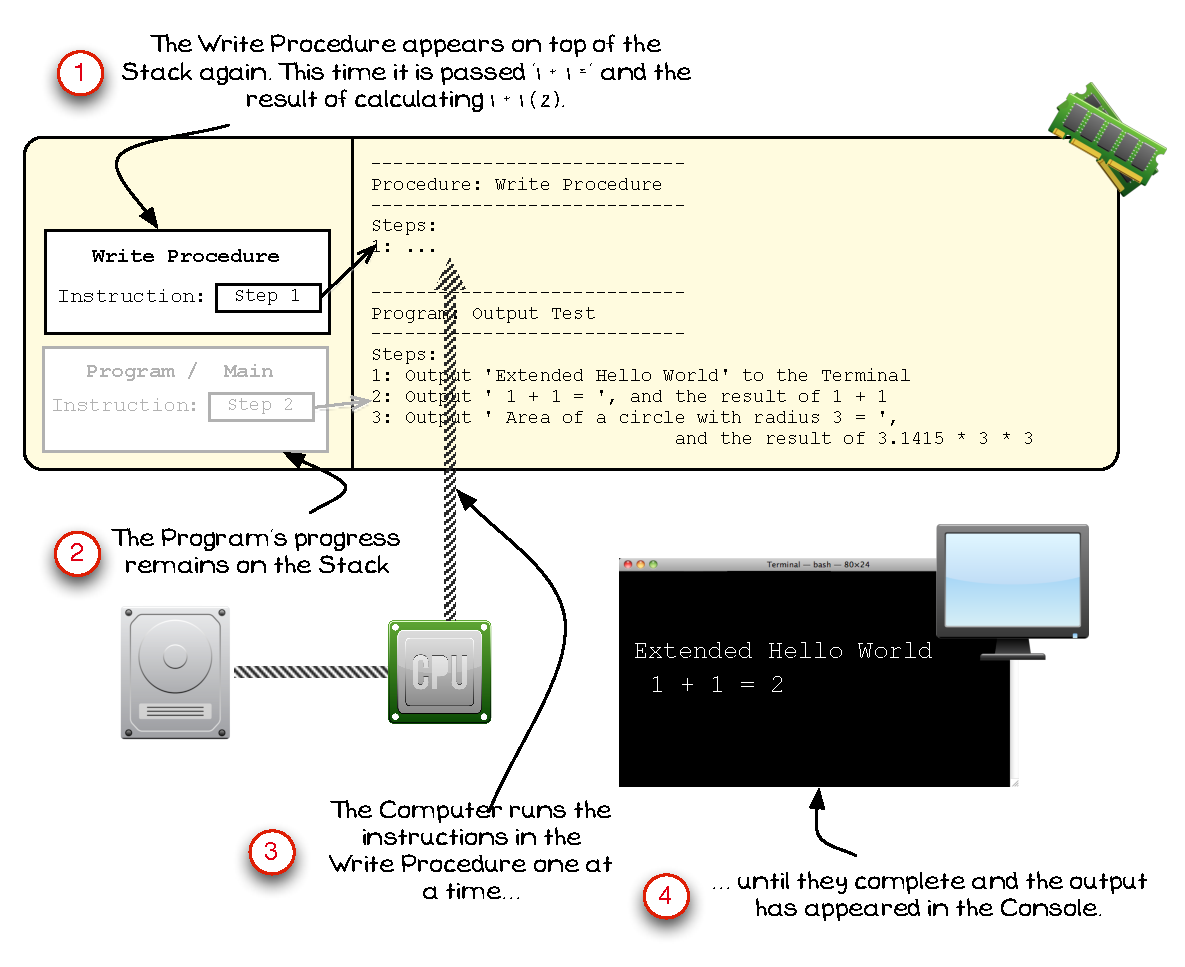
\includegraphics[width=\textwidth]{./topics/program-creation/images/ProgramExecution07} 
   \caption{The Write Procedure is called a second time}
   \label{fig:program-creation-visualise-helloworld-7}
\end{figure}

\mynote{
\begin{itemize}
  \item In Figure \ref{fig:program-creation-visualise-helloworld-7} the indicated areas show the following:
  \begin{enumerate}
    \item A new Frame is created for the Write Procedure. This allows the Computer to keep track of which statement is the current statement within this Procedure.
    \item The program's current instruction remains on the Stack for when the call to the Write procedure finishes.
    \item Each of the instructions in the Write procedure are executed to write the data to the Terminal.
    \item The output text appears on the Terminal.
  \end{enumerate}
\end{itemize}
}

% subsubsection the_second_call_to_write (end)
\clearpage
\subsubsection{The Second Write Call Ends} % (fold)
\label{ssub:the_second_write_call_ends}

When the second call to Write ends control returns to the Program, which moves on to its final instruction.

\begin{figure}[htbp]
   \centering
   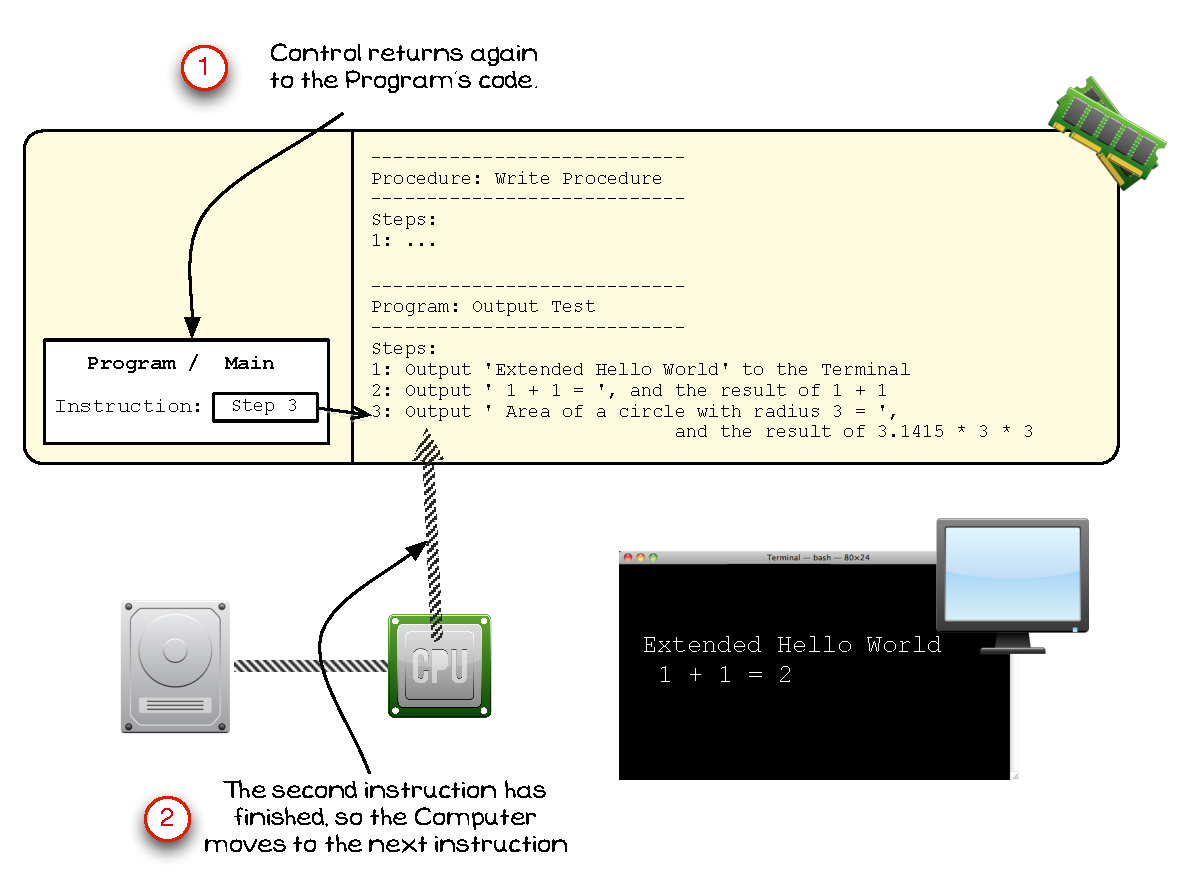
\includegraphics[width=\textwidth]{./topics/program-creation/images/ProgramExecution08} 
   \caption{The second call to the Write Procedure ends, and control returns to the Program}
   \label{fig:program-creation-visualise-helloworld-8}
\end{figure}

\mynote{
\begin{itemize}
  \item In Figure \ref{fig:program-creation-visualise-helloworld-8} the indicated areas show the following:
  \begin{enumerate}
    \item When the second call to the Write Procedure ends control returns to the program's code.
    \item As the second instruction has now finished the Computer moves to the third, and final, instruction in the program.
  \end{enumerate}
\end{itemize}
}

% subsubsection the_second_write_call_ends (end)
\clearpage
\subsubsection{The Third Call to Write} % (fold)
\label{ssub:third_call_to_write}

The final instruction in the program is a third call to the Write Procedure. 

\begin{figure}[htbp]
   \centering
   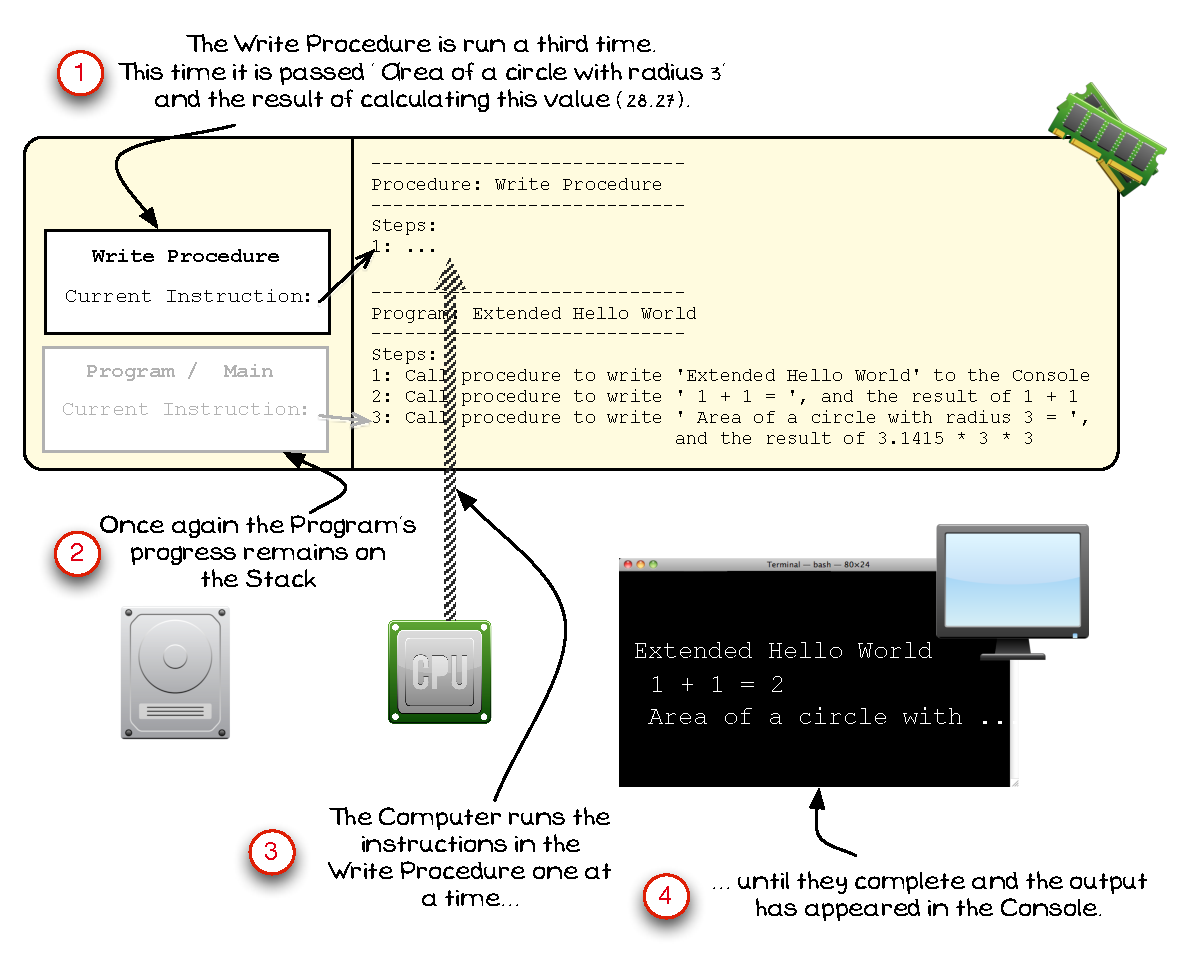
\includegraphics[width=\textwidth]{./topics/program-creation/images/ProgramExecution09} 
   \caption{The Write Procedure is called a third can final time}
   \label{fig:program-creation-visualise-helloworld-9}
\end{figure}

\mynote{
\begin{itemize}
  \item In Figure \ref{fig:program-creation-visualise-helloworld-9} the indicated areas show the following:
  \begin{enumerate}
    \item Once again, a Stack Frame is created to keep track of the progress within the Write Procedure.
    \item The program's current instruction remains on the Stack so that the Computer can return to it when the Write Procedure ends.
    \item Each of the instructions in the Write Procedure are executed.
    \item The Write Procedure writes the data passed to it to the Terminal.
  \end{enumerate}
\end{itemize}
}

% subsubsection third_call_to_write (end)
\clearpage
\subsubsection{The Program Ends} % (fold)
\label{ssub:program_ends}

When the last instruction in the Write Procedure finishes control return back to the Program, which has no more instructions. This means that the program has finished.

\begin{figure}[htbp]
   \centering
   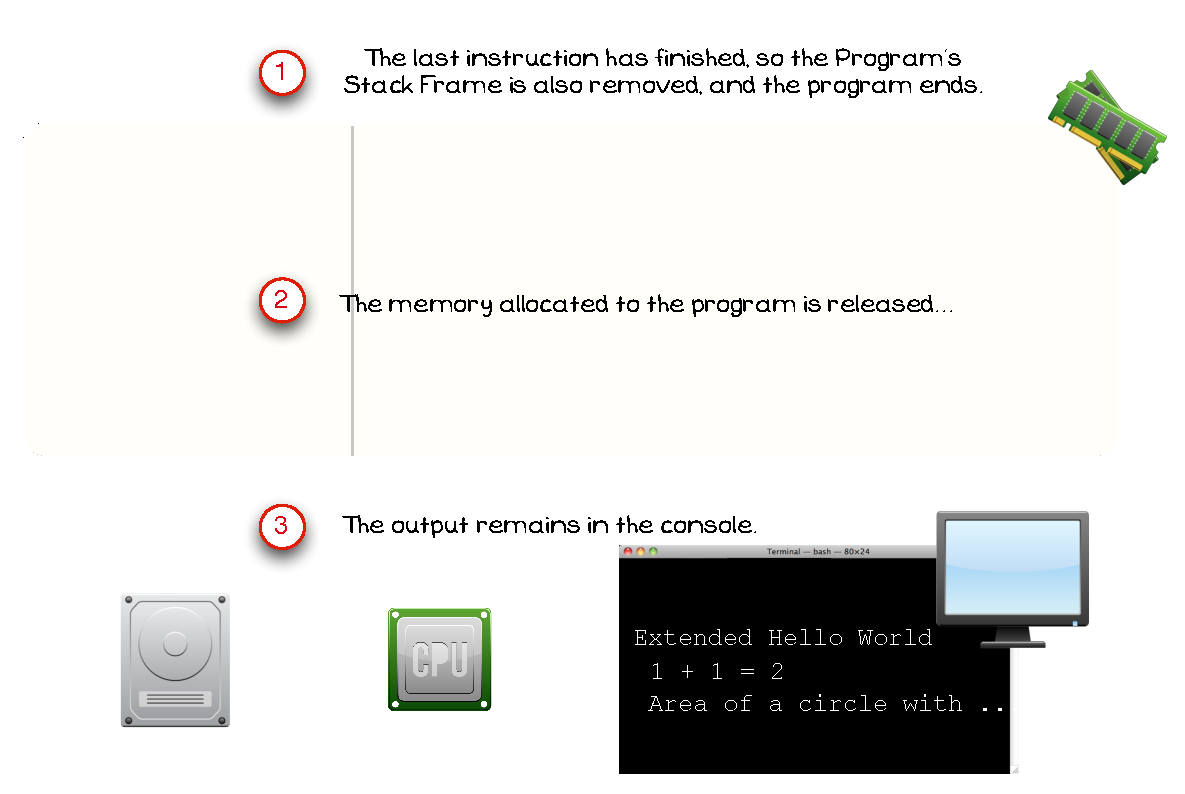
\includegraphics[width=\textwidth]{./topics/program-creation/images/ProgramExecution10} 
   \caption{The Write Procedure ends, then the program ends}
   \label{fig:program-creation-visualise-helloworld-10}
\end{figure}

\mynote{
\begin{itemize}
  \item In Figure \ref{fig:program-creation-visualise-helloworld-10} the indicated areas show the following:
  \begin{enumerate}
    \item The Write Procedure has finished its instructions, and so it ends. This was also the last instruction in the program's code, so it also ends. This tells the Operating System that Program has finished.
    \item The Operating System releases the memory used by the program so that it can be use by other programs.
    \item All of this will have happened in an instant, and after the program has finished all that remains is the output in the Terminal.
  \end{enumerate}
\end{itemize}
}

% subsubsection program_ends (end)

% subsection calling_a_procedure (end)
\clearpage
\subsection{Summary} % (fold)
\label{sub:program_creation_visualise_summary}

In this section you have seen the actions that occur behind the scenes when your program is executed. The most important aspects are the fact that the instructions run one at a time in \textbf{sequence}, and that a procedure call results in the instructions within the Procedure running until they end. Its also important to remember that the instructions within the Procedure must finish before control returns to where the call was made.

\bigskip

\mynote{
\begin{itemize}
  \item A Program is a sequence of instructions.
  \item These instructions are organised into Procedures that can be called. 
  \item The program's instructions are loaded into memory when the program is launched.
  \item Instructions are run one at a time.
  \item The Stack is used to keep track of the current instruction.
  \item When the program starts a Frame is added to the Stack to set the entry point as the first instruction.
  \item When a Procedure is called, a Frame is added to the Stack to keep track of its current instruction. 
\end{itemize}
}

% subsection summary (end)